% !TeX program = latexmk
% !TeX root = dp_puzzle.tex
% English master manuscript. Edit this file directly after the initial assembly.
% Chinese review counterpart: main.tex and sections/*.tex.
% Chapters are inline; tables, figures, and bibliography use shared sources.
\RequirePackage[T1]{fontenc}
\documentclass[conference,10pt,letterpaper]{IEEEtran}
\usepackage[no-math]{fontspec}
\setmainfont{TeX Gyre Termes}
\setsansfont{TeX Gyre Heros}
\setmonofont{TeX Gyre Cursor}
\usepackage{amsmath,amssymb}
\usepackage{graphicx}
\usepackage[caption=false,font=footnotesize]{subfig}
\usepackage{booktabs}
\usepackage{cite}
\usepackage[hidelinks]{hyperref}
\graphicspath{{figures/}}
\newcommand{\PaperTitle}{DP-Puzzle: Exploring Throughput Ratios in Multi-Precision Tensor Cores with Composable Dot-Product Units}
\title{\PaperTitle}
\author{\IEEEauthorblockN{Anonymous Submission}}
\hypersetup{pdfauthor={},pdftitle={\PaperTitle},pdfsubject={English manuscript}}
\newcounter{DACreferencepage}
\AtEndDocument{%
  \ifnum\value{page}>\value{DACreferencepage}\relax
    \PackageWarningNoLine{DAC2027}{References exceed one page}%
  \fi}
\begin{document}
\bstctlcite{DPBSTcontrol}
\maketitle

% Queue Table I at the top of the first page's right column.
\suppressfloats[t]
% Opening-page industrial-ratio overview; automatic caption numbering.
\begin{table}[t]
\centering
\caption{Per-device dense matrix peaks (PFLOP/s) and roadmap targets.}
\label{tab:vendor_ratios}
\begingroup\footnotesize\setlength{\tabcolsep}{2pt}
\begin{tabular*}{\columnwidth}{@{\extracolsep{\fill}}llrrrl@{}}
\toprule
Vendor & Product & BF16 & MXFP8 & MXFP4 & Ratio \\
\midrule
NVIDIA & B200 SXM~\cite{nvidiahgx}
 & 2.250 & 4.500 & 9.000 & $1:2:4$ \\
 & B300 SXM~\cite{nvidiahgx}
 & 2.250 & 4.500 & 13.500 & $1:2:6$ \\
 & Rubin GPU~\cite{nvidiaverarubin}
 & 4.000 & 17.500 & 35.000 & $\approx 1:4:8$ \\
\midrule
AMD & MI355X~\cite{amdmi355x}
 & 2.517 & 5.033 & 10.066 & $1:2:4$ \\
 & MI455X~\cite{amdmi455x}
 & 5.033 & 20.133 & 40.265 & $1:4:8$ \\
\midrule
Huawei & Ascend 950PR~\cite{huawei950}
 & 0.432 & 0.865 & 1.730 & $1:2:4$ \\
 & Ascend 960PR$^\dagger$~\cite{huawei960roadmap}
 & 1.000 & 2.000 & 8.000 & $1:2:8$ \\
\bottomrule
\end{tabular*}
\par\smallskip
\parbox{\columnwidth}{\raggedright
Ratios are normalized to BF16 peaks
$\dagger$ denotes an R\&D roadmap target.}
\endgroup
\end{table}


% BEGIN REVIEW PAIR: 00_abstract.tex
\begin{abstract}
Multi-precision tensor hardware must balance high- and low-precision throughput within a limited area budget. The same ratio can be realized by extending the reduction dimension K or by adding independent outputs along N, with different circuit and data-supply costs. DP-Puzzle shares arithmetic across a lane--group--DP hierarchy and uses specialized E and QE components to construct $1:2:6$, $1:2:8$, and $1:4:8$ ratios. Synthesis and activity-based power analysis of six DPs at 12\,nm and 1\,GHz show that K expansion reduces component area by 0.65\%--2.40\% and estimated low-precision active power by 2.02\%--3.97\% relative to N composition at matched peak throughput. Bandwidth analysis separates input reuse from accumulator capacity and output-port demand. Under a fixed core-area budget, all four K ratios occupy distinct latency- and energy-optimal regions of the H/Q/E workload space. Prefill workloads derived from three DeepSeek models favor $1:4:8$ under the reference W4A8 mapping, whereas FP4 experts and long contexts can shift some workloads toward $1:2:8$. These results connect dot-product circuit costs to mixed-precision compute demand for workload-driven ratio selection.
\end{abstract}
\begin{IEEEkeywords}
Composable Dot-Product Architecture, Multi-Precision Tensor Cores, Throughput Ratios, Hardware Cost--Performance Trade-offs
\end{IEEEkeywords}
% END REVIEW PAIR: 00_abstract.tex

% BEGIN REVIEW PAIR: 01_introduction.tex
\section{Introduction}
\label{sec:introduction}
Growing model sizes and computational demands have made lower-precision numerical formats a common optimization for large AI models~\cite{deepseekv3}. General matrix multiplication (GEMM) accounts for much of their computation, and its execution formats have progressively shifted from single-precision floating point (FP32) toward lower precisions, including TensorFloat-32 (TF32), half precision (FP16), and BF16. Advances in quantization have also made FP8, INT8, FP6, FP4, and microscaling formats~\cite{ocpmx2023} with shared scaling factors important options for inference. DeepSeek-V4.1-Flash~\cite{deepseekv41source}, for example, uses mixed-precision GEMMs: mixture-of-experts (MoE) computation and most attention projections use FP8, the QK path of the sparse attention indexer uses MXFP4, and the main attention QK/PV computations use BF16. These workloads require inference hardware to support multiple precisions within the same model.

For a fixed input bit width, lower-precision formats allow more elements to be supplied in parallel, motivating the conventional BF16:MXFP8:MXFP4 peak throughput ratio of $1:2:4$. Recent commercial AI chips depart from this ratio by selectively increasing FP4 throughput or increasing both FP8 and FP4 throughput, as summarized in Table~\ref{tab:vendor_ratios}. Model development, however, proceeds on a different timescale from chip design and manufacturing. A chip tailored to current model requirements may therefore be poorly matched to future workloads. Tensor cores, which provide much of an AI chip's compute throughput, must support multiple precisions while allocating relative throughput across them. This allocation must balance hardware cost against the demands of both current and future models.

We present DP-Puzzle to connect the hardware cost of throughput-ratio choices to their benefits for evolving model workloads. Tensor cores typically organize dot-product units into two-dimensional arrays with systolic~\cite{jouppi2017tpu} or broadcast dataflows. We therefore focus on dot-product units that support multiple formats and allow low-precision throughput to be increased independently. We characterize their area and power using Synopsys synthesis and power analysis at 12\,nm and 1\,GHz, then construct a chip-level throughput model under common area and power constraints. Six precision-migration scenarios represent possible changes in future workloads, allowing us to evaluate the estimated GEMM compute-latency benefits of nine throughput ratios.

% Promoted from the approved temporary manuscript.
\suppressfloats[t]
\begin{table}[t]
\centering
\caption{精度支持与组合式配比配置能力。}
\label{tab:related_features}
\begingroup\footnotesize\setlength{\tabcolsep}{1pt}
\def\Y{$\checkmark$}\def\N{$\times$}\def\E{$\triangle$}
\begin{tabular*}{\columnwidth}{@{\extracolsep{\fill}}l*{10}{c}@{}}\toprule
Design & TF32 & FP16 & BF16 & \shortstack{MX\\FP8} & \shortstack{MX\\FP6} & \shortstack{MX\\FP4} & INT8 & \shortstack{NV\\FP4} & HiF4 & \shortstack{Multi\\Ratio} \\\midrule
Ten-Four~\cite{rout2026tenfourv3} & \Y & \Y & \Y & \Y & \N & \N & \Y & \N & \N & \N \\
MXDOTP~\cite{islamoglu2025mxdotp} & \N & \N & \N & \Y & \N & \N & \N & \N & \N & \N \\
FPnew~\cite{mach2021fpnew} & \N & \Y & \Y & \E & \N & \N & \N & \N & \N & \N \\
MiniFloats~\cite{bertaccini2024minifloats} & \N & \Y & \Y & \E & \N & \N & \N & \N & \N & \N \\
TransDot~\cite{transdot2026} & \N & \Y & \N & \E & \N & \E & \N & \N & \N & \N \\
\midrule
DP-Puzzle & \Y & \Y & \Y & \Y & \Y & \Y & \Y & \Y & \Y & \Y \\
\bottomrule\end{tabular*}
\par\smallskip
\parbox{\columnwidth}{\raggedright
$\checkmark$: supported; $\times$: absent in the reported configuration; $\triangle$: element arithmetic supported, integrated MX scaling not established. FPnew and MiniFloats also support FP32/FP64; MiniFloats uses FP8 E5M2/E4M3 and BF16-encoded FP16alt.}
\endgroup
\end{table}


Our contributions are as follows:
\begin{enumerate}
\item \textbf{Composable multi-precision datapaths:} DP-Puzzle combines shared dot-product arithmetic with FP8-only, FP4-only, and shared FP8/FP4 units to adjust throughput ratios while retaining support for TF32, FP16/BF16, INT8, MXFP8/6/4, NVFP4, and HiF4. Relative to \mbox{$1:2:4$}, the \mbox{$1:2:8$} configuration doubles MXFP4 throughput with a 33.60\% area increase, improving MXFP4 area and energy efficiency by 49.70\% and 27.27\%, respectively.
\item \textbf{Chip-level throughput modeling:} Synthesis and power analysis driven by Qwen3-8B~\cite{qwen3technicalreport} data at 12\,nm and 1\,GHz characterize nine dot-product configurations. These costs determine deployable core counts and absolute peak throughput for each precision under joint area and compute-power budgets, quantifying how low-precision expansion trades per-unit throughput against chip-level deployment density.
\item \textbf{Workload-driven ratio selection:} Six current and prospective precision scenarios for DeepSeek-V4.1-Flash, evaluated over 1K--1M contexts, connect workload migration to estimated GEMM compute latency. Adding a matched compute-power budget shifts the best aggregate ratio from \mbox{$1:8:16$} to \mbox{$1:2:8$}, yielding a modeled $1.147\times$ speedup over \mbox{$1:2:4$} across equally weighted scenarios. Moderate expansion thus balances remaining high-precision demand with future low-precision workloads.
\end{enumerate}

The rest of this paper is organized as follows. Section~\ref{sec:background} presents the background and motivation. Section~\ref{sec:architecture} describes the shared multi-precision microarchitecture, Group specialization, and throughput-ratio composition. Section~\ref{sec:evaluation} presents the evaluation methodology and hardware cost results. Section~\ref{sec:workload} analyzes workload-driven throughput-ratio selection. Section~\ref{sec:conclusion} concludes the paper.


% END REVIEW PAIR: 01_introduction.tex

% BEGIN REVIEW PAIR: 02_background.tex
\section{Background and Motivation}
\label{sec:background}

\subsection{Floating-Point and Microscaling Formats}
\label{sec:formats}

Floating-point formats encode a sign, an exponent, and a fraction. The exponent width determines dynamic range, whereas the fraction width determines relative precision. TF32 retains FP32's exponent range with a shorter significand to reduce the cost of tensor computation; FP16 and BF16 favor precision and dynamic range, respectively~\cite{burgess2019bfloat16}. The Open Compute Project (OCP) microscaling (MX) formats~\cite{ocpmx2023} represent each element as $x_{j,i}=X_jP_{j,i}$, where $X_j$ is a shared block scaling factor and $P_{j,i}$ is the decoded element value. MXFP8, MXFP6, and MXFP4 use E5M2/E4M3, E3M2/E2M3, and E2M1 element encodings, respectively. All three share one E8M0 scale across 32 elements to extend the representable range.

Quantizing both weights and activations to MXFP4, however, can incur substantial accuracy loss. The power-of-two restriction of its E8M0 scale is a major source of quantization error~\cite{egiazarian2026bridging,zhang2026benchmarking}. To improve quantization accuracy, NVFP4 retains E2M1 elements, reduces the block size to 16, and combines an E4M3 block scale with an FP32 tensor scale~\cite{nvidia2024nvfp4}. HiF4 instead uses S1P2 fixed-point elements and hierarchical micro-exponent scaling to balance within-block dynamic range and precision~\cite{hifloat4}. Both MX-like formats use scales with fractional significand bits, introducing additional significand-multiplication hardware.

\subsection{Tensor Computation with Dot-Product Units}
\label{sec:tensor_organization}

Dot-product accumulation for conventional and microscaling formats~\cite{ocpmx2023} can be expressed as
\begin{equation}
\begin{aligned}
\operatorname{DP}_K(\mathbf{a},\mathbf{b},c)
&=c+\sum_{k=0}^{K-1}a_kb_k \\
&=c+\sum_{j=0}^{G_s-1}
\widetilde{X}_j^{(A)}\widetilde{X}_j^{(B)}
\underbrace{\sum_{i=0}^{g-1}
P_{j,i}^{(A)}P_{j,i}^{(B)}}_{q_j},
\end{aligned}
\label{eq:blockdot}
\end{equation}
The two inputs use the same scaling-block boundaries along the reduction dimension. Here, $g$ is the block size, $G_s=\lceil K/g\rceil$, and the final block is zero-padded. The term $q_j$ is the dot product within block $j$, and $\widetilde{X}_j$ is its effective scale. For conventional floating-point formats, $\widetilde{X}_j=1$ and $P_{j,i}$ is the original element value; for MX formats, $\widetilde{X}_j=X_j$. HiF4's local micro-exponents are incorporated into $P_{j,i}$.

\subsection{Related Work on Multi-Precision Dot-Product Design and Design-Space Exploration}
\label{sec:datapath_sharing}

For multiplier reuse, Bit Fusion composes low-bit-width multiplication units through shifts and additions~\cite{bitfusion2018}. Park et al. share multipliers and reduction datapaths between FP16 significand multiplication and INT8/INT4 dot products~\cite{parkMultimode8KMACHWutilizationaware2022}. Abdel-Aziz et al. support higher precision through temporal decomposition and analyze the overhead of floating-point exponent alignment and addition~\cite{abdelaziz2021overheads}. For multi-format computation and fused reduction, FPnew supports multiple floating-point operations through configurable format slices~\cite{mach2020fpnew}. MiniFloats fuses two low-precision products with a higher-precision addend, reducing repeated normalization and rounding~\cite{bertaccini2022minifloat}. TransDot reuses multiplier partial products and partitionable shifters~\cite{transdot2026}; Ten-Four connects dot products in multiple formats to a shared reduction backend~\cite{rout2026tenfourv3}. MXDOTP uses a unified internal element representation, integrates MX scaling into the dot-product datapath, and accumulates in FP32~\cite{islamoglu2025mxdotp}.

For alignment and accumulation, a dynamic alignment anchor selects a reference exponent from the inputs. A fixed anchor instead uses a reference determined by the format's exponent range, trading a wider fixed-point datapath for simpler exponent-selection logic. Products can be aligned and reduced together with the addend $C$, or a floating-point adder can combine $C$ with the scaled dot product. Where $C$ enters the datapath determines the alignment range and accumulation overhead~\cite{bertaccini2022minifloat,lutzFusedFP84Way2024}. Internal accumulation order, truncation positions, and rounding rules jointly determine numerical results~\cite{sun2023tensorcores,xie2025mmasim}. In design-space exploration, Crafton et al. and MX-Like further examine trade-offs among low-precision formats, compute organization, and hardware cost~\cite{paretomac2025,zhao2026mxlike}, but neither addresses throughput-ratio selection.

Table~\ref{tab:related_features} compares the precision formats supported by DP-Puzzle and related dot-product designs. Building on support for multiple formats, our design adds specialized low-precision units to adjust the relative peak throughputs within each dot-product unit, enabling multiple throughput ratios.

\subsection{Motivation for Throughput-Ratio Exploration}
\label{sec:commercial_ratios}
\label{sec:ratio_motivation}

Table~\ref{tab:vendor_ratios} summarizes recent products and development roadmaps from major GPGPU and NPU vendors, illustrating industry interest in $1:2:6$, $1:4:8$, and $1:2:8$ ratios. These disclosures do not explain the rationale for selecting each ratio, and the configurations cover only a small part of the design space. We therefore extend the exploration to $1:4:4$, $1:2:12$, $1:2:16$, $1:6:12$, and $1:8:16$. Together with the three ratios above and the $1:2:4$ baseline, these form a design space of nine candidates. Our objective is to determine how hardware cost should be traded against performance benefits as the precision requirements of future model workloads evolve.
% END REVIEW PAIR: 02_background.tex

% BEGIN REVIEW PAIR: 03_architecture.tex
\section{Composable Dot-Product Microarchitecture for Throughput-Ratio Exploration}
\label{sec:architecture}
\label{sec:brick_definition}

Fig.~\ref{fig:dp_architecture} shows the $1:2:4$ baseline datapath of DP-Puzzle, organized into three levels: Lane, Group, and dot-product unit (DP). Each Lane shares multiplication and local reduction across precisions. Each Group incorporates block scaling and produces a unified partial-sum representation, while the DP performs global alignment and accumulation. Adding specialized low-precision Groups to this baseline yields DP designs with different throughput ratios.

\subsection{Notation and Architecture Overview}
\label{sec:notation_conventions}

We use T, H, Q, and E to denote TF32, FP16/BF16, MXFP8/6, and MXFP4/NVFP4/HiF4, respectively. Fixed-point values use $\mathrm{Q}I.F$ and $\mathrm{UQ}I.F$ notation for signed two's-complement and unsigned representations. Here, $I$ is the number of integer bits excluding the sign bit, and $F$ is the number of fractional bits; the total widths are $1+I+F$ and $I+F$, respectively~\cite{ti2003qformat}.

Compute parallelism is denoted by $\mathrm{T}x_T\mathrm{H}x_H\mathrm{Q}x_Q\mathrm{E}x_E$, where $x_p$ is the number of element pairs processed per cycle in precision mode $p$; the modes are mutually exclusive. A baseline Lane supports T1H2Q4E8, two Lanes form a T2H4Q8E16 Group, and four Groups form a T8H16Q32E64 DP. The DP also supports 32 INT8 products per cycle with INT32 accumulation. At a fixed array size and clock frequency, the H:Q:E throughput ratio therefore equals the ratio of their respective parallelisms within each DP.

\begin{figure}[t]
\centering
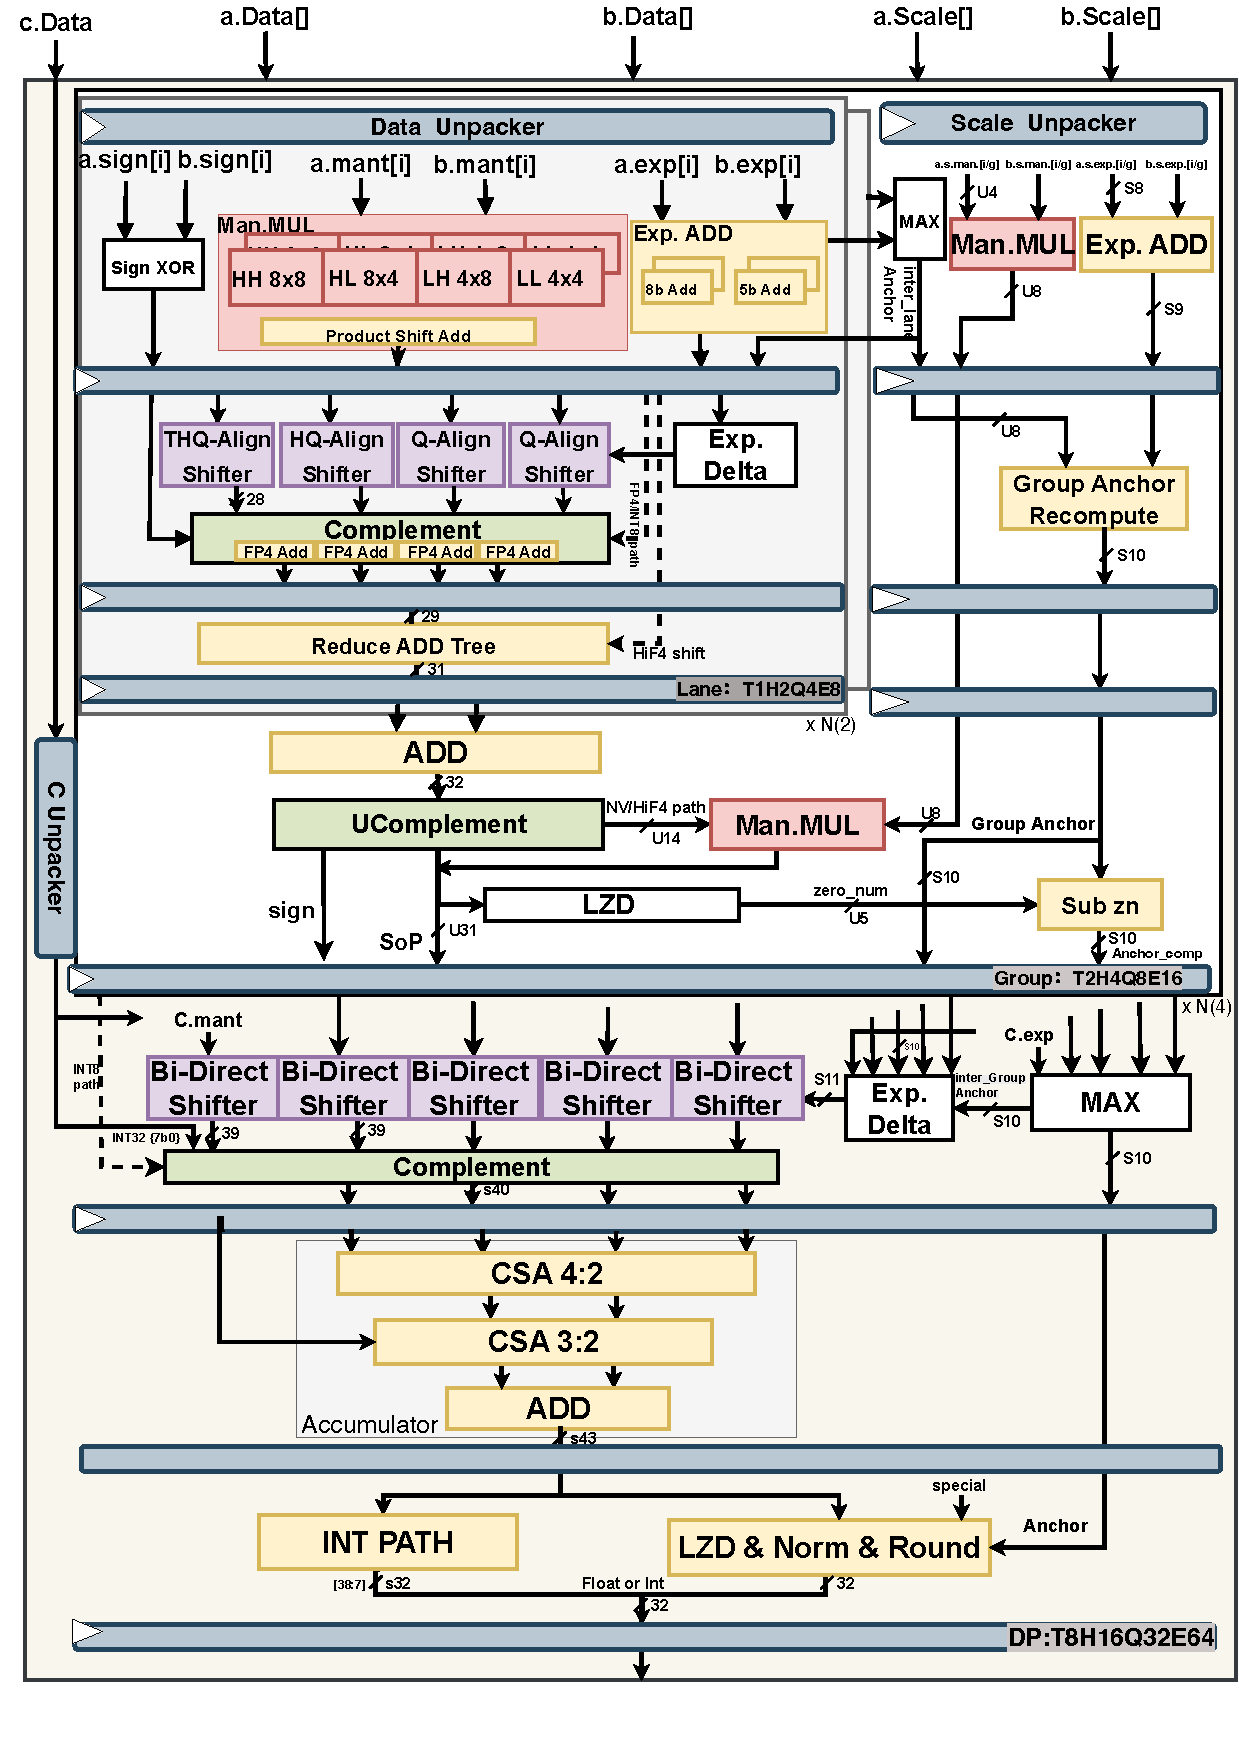
\includegraphics[width=\columnwidth]{baseline_arch.pdf}
\caption{DP-Puzzle's $1:2:4$ baseline microarchitecture. Each T2H4Q8E16 Group contains two shared multi-precision Lanes, and four Groups form a T8H16Q32E64 DP. Other throughput ratios are constructed by adding specialized low-precision Groups.}
\label{fig:dp_architecture}
\end{figure}

\subsection{Lane: Shared Multi-Precision Arithmetic}
\label{sec:unpack_recode}
\label{sec:full_brick}

Each Lane provides T1H2Q4E8 parallelism, matching the eight-element sharing granularity of HiF4's second-level micro-exponent. During decoding (Fig.~\ref{fig:data_unpack}), T/H operands are separated into exponents and significands, while Q operands are mapped exactly to an internal E5M3 representation. MXFP4/NVFP4 and HiF4 with its first-level micro-exponent incorporated are mapped to UQ3.1 and UQ2.2, respectively. These four-bit fixed-point magnitudes absorb the element exponents. All formats, including INT8, separate signs from magnitudes to share unsigned multipliers.

\begin{figure}[t]
\centering
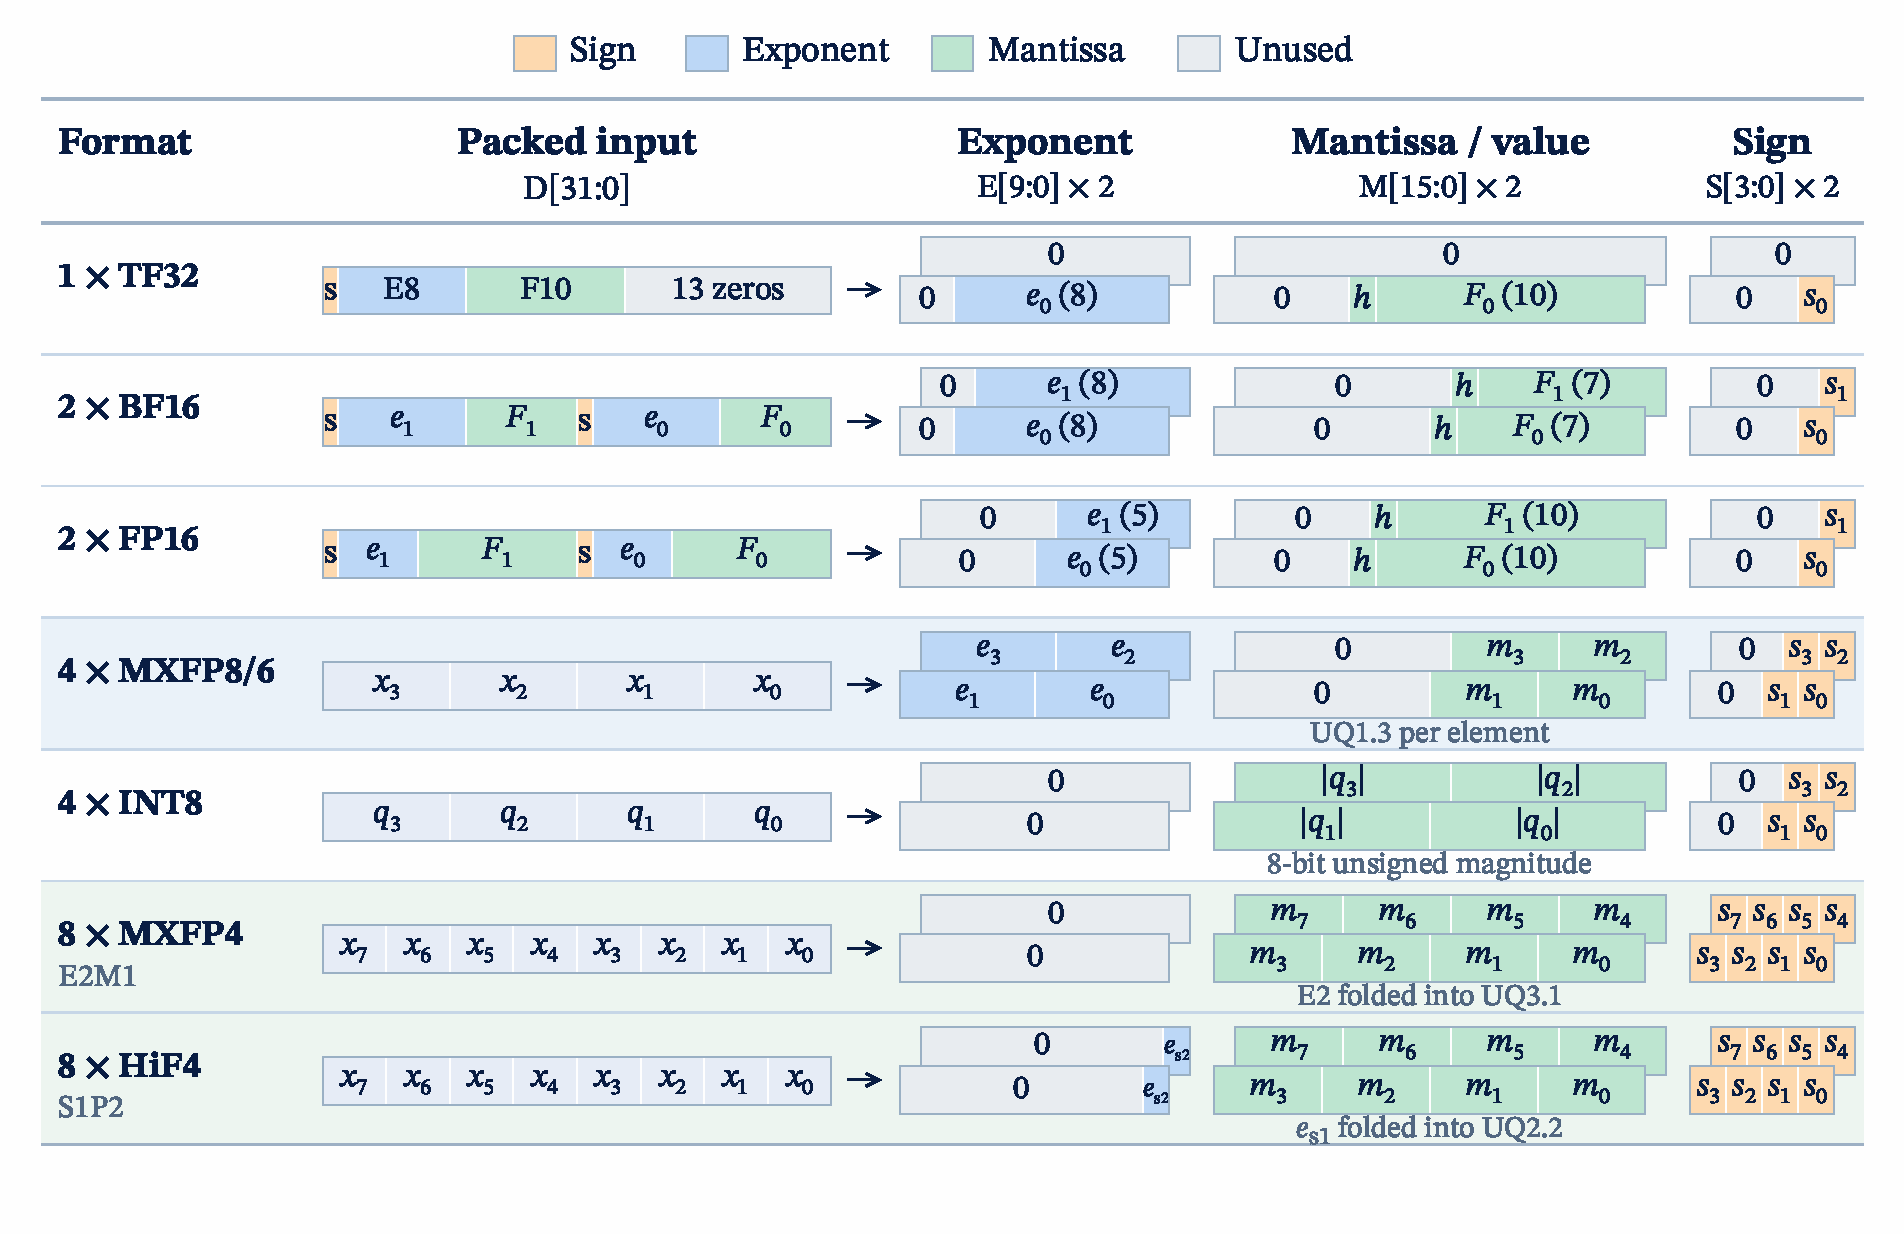
\includegraphics[width=\columnwidth]{unpack_layout.pdf}
\caption{Mapping input formats to shared exponent, significand, and sign fields.}
\label{fig:data_unpack}
\end{figure}

Each Lane contains two multiplier sets, each comprising one $8\times8$, one $8\times4$, one $4\times8$, and one $4\times4$ unit. For TF32/FP16, the 11-bit significands are split into upper and lower portions, with four bits in the latter: $a=2^4a_h+a_l$ and $b=2^4b_h+b_l$. The product is reconstructed from partial products as
\begin{equation}
ab=2^8a_hb_h+2^4(a_hb_l+a_lb_h)+a_lb_l.
\label{eq:mantissa_reuse}
\end{equation}
TF32 and FP16 activate one and two sets, respectively; BF16 uses only the $8\times8$ unit in each set. Q computes two independent four-bit products per set, whereas E uses all four units. INT8 uses one $8\times8$ unit per set and reconstructs a second eight-bit product from the cross partial products.

% Precision reference: MMA-Sim v3, Table III (Blackwell UTCQMMA) and Algorithm 7.
T/H/Q use one, two, and four shared unsigned right shifters, respectively, to align products to the maximum valid product exponent within the Group. Guided by reverse engineering of Blackwell FP8 arithmetic~\cite{xie2025mmasim}, we use a UQ2.26 alignment window with 26 fractional bits. Magnitudes are right-shifted before conversion to two's complement, implementing truncation toward zero. E/INT8 bypass the wide shifters. E's eight products are converted to signed values and reduced pairwise to four terms; INT8's four terms enter directly. All modes share a balanced four-input adder tree that produces a 31-bit signed partial sum. HiF4's second-level micro-exponent is incorporated by shifting the Lane sum.

\subsection{Group: Scale-Factor Integration and Unified Partial Sums}

Two Lanes form a T2H4Q8E16 Group, matching NVFP4's 16-element scaling block; larger blocks broadcast the same scale factor across Groups. The Group first combines the Lane results and separates the sign and magnitude, then applies the shared scale factors. Only NVFP4/HiF4 require scale-significand multiplication. The two four-bit scale significands are premultiplied into an eight-bit coefficient. After removing structurally zero low-order bits, the 14-bit Group magnitude is multiplied by this coefficient using a shared $14\times8$ multiplier. The resulting 22-bit value is mapped to the U31 magnitude interface. MX's E8M0 scale factors contribute only to the exponent.

% Layout cross-check: dp-top-v1.8.md, dp_group.v and dp_functions.vh;
% the v1.8 HiF4 path uses the NVFP4 fractional layout after Lane-local e2 fusion.
The U31 interface has $F_p=28/27/26$ fractional bits for T/H/Q and 21 and 19 fractional bits for MXFP4 and NVFP4/HiF4, respectively. Let $E_{\mathrm{loc}}$ denote the unbiased local alignment exponent and $E_{\mathrm{scale}}$ the sum of the two unbiased scale exponents. The exponent associated with the most significant physical bit of the magnitude is
\begin{equation}
\mathrm{Anchor}_{\mathrm{raw}}
=E_{\mathrm{loc}}+E_{\mathrm{scale}}+30-F_p.
\label{eq:anchor_recompute}
\end{equation}
For E, the element exponents and micro-exponents are already incorporated into the magnitude, so $E_{\mathrm{loc}}=0$. Formats without block scaling use $E_{\mathrm{scale}}=0$. This exponent calculation proceeds in parallel with significand reduction.

For finite nonzero magnitudes, leading-zero detection (LZD) produces a count $z$ and the exponent of the most significant nonzero bit, $\mathrm{Anchor}_{\mathrm{eff}}=\mathrm{Anchor}_{\mathrm{raw}}-z$. Each Group outputs the U31 magnitude without normalization shifts, a separate sign, and both exponent coordinates.

\subsection{DP: Shared Alignment and Fused Accumulation}

The DP introduces the addend $C$ after within-Group reduction and scale-factor integration. It determines the global reference exponent $E_{\mathrm{max}}$ from the Group comparison exponents and the decoded exponent of $C$. Left-shifting a Group magnitude by $z$ bits for normalization and then right-shifting it for alignment gives the net shift
\begin{equation}
\begin{aligned}
\Delta&=z-(E_{\mathrm{max}}-\mathrm{Anchor}_{\mathrm{eff}})\\
      &=\mathrm{Anchor}_{\mathrm{raw}}-E_{\mathrm{max}}.
\end{aligned}
\label{eq:net_alignment_shift}
\end{equation}
After zero-padding the original magnitude to a 39-bit window, a single bidirectional shift suffices; right shifts truncate toward zero. Signs are restored before summation through a carry-save adder (CSA) compression tree and a single carry-propagate adder (CPA). The result is then normalized and rounded to FP32 using round-to-nearest, ties-to-even.

INT8/INT32 bypass floating-point alignment and output normalization while sharing the accumulation datapath. Registers are enabled according to the request's precision. All configurations retain an eight-cycle latency and a throughput of one independent request per cycle.

\subsection{Group Specialization and Throughput-Ratio Composition}
\label{sec:specialized_midgroups}
\label{sec:expansion}

Specialization preserves the numerical mappings, precision, and rounding rules of supported formats while removing decoding and arithmetic for unsupported formats. Each Lane in a Q8E16 Group uses eight $4\times4$ multipliers; Q activates four, whereas E activates all eight. It retains Q's 28-bit alignment path, the 31-bit Lane output, and E's scale-significand multiplication. Q8 retains only four $4\times4$ multipliers per Lane and removes E decoding, micro-exponent processing, and scale-significand multiplication. E8M0 scale factors contribute only to exponent updates.

E16 further reduces the alignment and reduction hardware. Each Lane retains eight $4\times4$ multipliers but removes element-exponent comparison, local alignment-reference generation across Lanes, and wide shifters. A narrow adder tree performs reduction, with HiF4's second-level micro-exponent incorporated after local summation; the Lane output is reduced to 14 signed bits. Combining two Lanes produces a 15-bit Group sum. Scaling and LZD operate on a 22-bit result, which is mapped to the common U31 magnitude and Anchor interface. E16 expansion therefore avoids the cost of Q's wide alignment and reduction paths.

Table~\ref{tab:ratio9_composition} lists the Group compositions of the nine DP configurations. Each retains four baseline multi-precision Groups and adds Q8, E16, or Q8E16 Groups to adjust low-precision throughput. Added Groups process additional $K$ segments for the same output, with scale factors distributed according to the original quantization-block boundaries.

% Group counts follow src/spec/dp/dptop/ mixed, Q-only, E192/E256,
% and QE192/QE256 expansion contracts. Ratios are normalized to H16.
% Single table source shared by the official and review manuscripts.
\begin{table}[t]
\centering
\caption{Group composition of the nine DP configurations.}
\label{tab:ratio9_composition}
\begingroup
\footnotesize
\setlength{\tabcolsep}{2pt}
\begin{tabular*}{\columnwidth}{@{\extracolsep{\fill}}lrrrrl@{}}
\toprule
H:Q:E & \shortstack{Baseline\\T2H4Q8E16} & Q8 & E16 & Q8E16 & \shortstack{Total DP\\parallelism} \\
\midrule
$1:2:4$  & 4 & 0 & 0  & 0  & T8H16Q32E64   \\
$1:2:6$  & 4 & 0 & 2  & 0  & T8H16Q32E96   \\
$1:2:8$  & 4 & 0 & 4  & 0  & T8H16Q32E128  \\
$1:4:4$  & 4 & 4 & 0  & 0  & T8H16Q64E64   \\
$1:4:8$  & 4 & 0 & 0  & 4  & T8H16Q64E128  \\
$1:2:12$ & 4 & 0 & 8  & 0  & T8H16Q32E192  \\
$1:2:16$ & 4 & 0 & 12 & 0  & T8H16Q32E256  \\
$1:6:12$ & 4 & 0 & 0  & 8  & T8H16Q96E192  \\
$1:8:16$ & 4 & 0 & 0  & 12 & T8H16Q128E256 \\
\bottomrule
\end{tabular*}
\par\smallskip
\parbox{\columnwidth}{\raggedright
Group columns count instances; H:Q:E denotes the peak throughput ratio.
Total DP parallelism counts element pairs per cycle in mutually exclusive
T/H/Q/E modes.}
\endgroup
\end{table}


The DP adds bidirectional shifters for the new Groups, extends exponent comparison, and widens accumulation so that all participating sources align to a common reference. As shown in Fig.~\ref{fig:dp_csa_expansion}, a 4:2 CSA network compresses the added results into two rows. A further 4:2 CSA merges these with the two baseline rows, which already include the single $C$ contribution. When only two Groups are added, their results enter the merge stage directly. A precision-controlled multiplexer (MUX) selects either the baseline or merged sum/carry pair for the shared CPA. Q8, E16, and Q8E16 participate in Q, E, and Q/E modes, respectively. When expansion is inactive, the MUX selects the baseline path, and the added Groups are excluded from exponent comparison and special-value reduction, preserving the original high-precision results.

\begin{figure}[t]
\centering
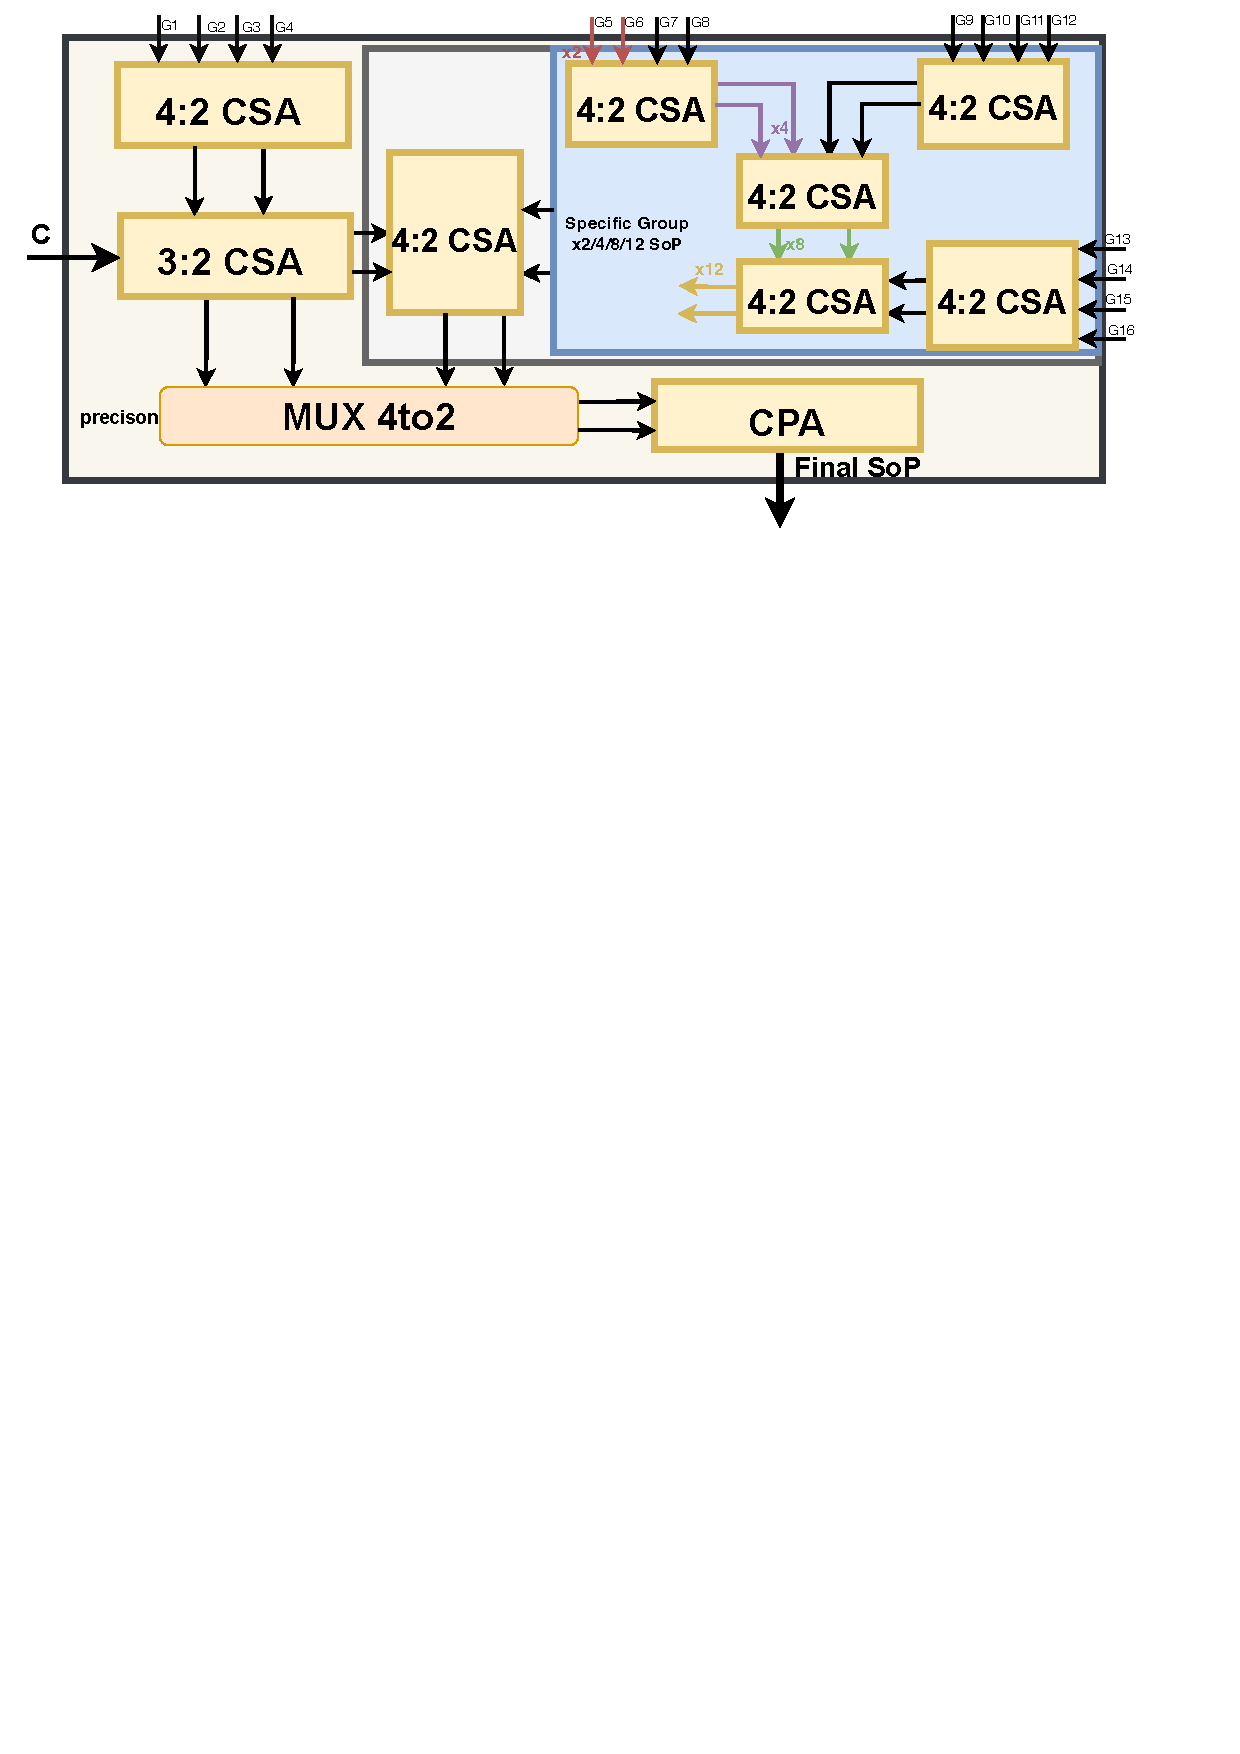
\includegraphics[width=\columnwidth]{dynamic_add.pdf}
\caption{Accumulation network for low-precision expansion. Results from 2/4/8/12 added Groups are merged with the baseline into sum and carry rows. A precision-controlled MUX selects the baseline or merged pair for the shared final CPA.}
\label{fig:dp_csa_expansion}
\end{figure}

This composition maps throughput-ratio choices to the addition of specialized Groups. The next section compares the area and power of the nine configurations at the same process node and frequency, providing the hardware costs for chip-level throughput-ratio exploration.
% END REVIEW PAIR: 03_architecture.tex

% BEGIN REVIEW PAIR: 04_evaluation.tex
\section{Evaluation}
\label{sec:evaluation}

\subsection{Experimental Setup and Verification}
\label{sec:eval_setup}
\label{sec:numerical_validation}

We implement the nine dot-product configurations in Verilog RTL and verify their functionality using Verilator. All designs are synthesized and analyzed for timing using Synopsys Design Compiler in TSMC 12\,nm technology at the TT corner (0.7\,V, 85$^\circ$C), targeting 1\,GHz with integrated clock gating enabled. The designs meet timing and electrical constraints. Area includes combinational logic, pipeline registers, and clock-gating cells. For power evaluation, we collect activations and weights from the first-layer MLP down-projection of Qwen3-8B running on WikiText-2~\cite{qwen3technicalreport,merity2016pointer}, and quantize them to BF16, MXFP8 E4M3, and MXFP4 E2M1. Power Compiler estimates total power using steady-state switching activity extracted from gate-level simulation at 1\,GHz. Area and power results correspond to synthesized dot-product units before clock-tree synthesis and place-and-route.

\subsection{Baseline Comparison with Prior Multi-Precision Units}
\label{sec:related_dp_evaluation}

% Generated by scripts/build_related_native.py; official manuscript.
\begin{table*}[t]
\centering
\caption{已有单元与 DP-Puzzle 的原工艺实现条件及效率。}
\label{tab:related_dp}
\begingroup\footnotesize\setlength{\tabcolsep}{1.5pt}
\def\Eff#1{\begin{tabular}{@{}lr@{}}#1\end{tabular}}
\begin{tabular*}{\textwidth}{@{\extracolsep{\fill}}l*{8}{c}@{}}\toprule
Metric & Ten-Four~\cite{rout2026tenfourv3} & MPICC~\cite{huangMPICCMultiplePrecisionInterCombined2025} & MXDOTP~\cite{islamoglu2025mxdotp} & FPnew~\cite{mach2021fpnew} & MiniFloats~\cite{bertaccini2024minifloats} & TransDot~\cite{transdot2026} & \multicolumn{2}{c}{DP-Puzzle} \\
\cmidrule(lr){8-9}
 & & & & & & & $1:2:4$ & $0:2:4$ \\
\midrule
Structure & Fused DP & $n$-term MAC & MX DP & SIMD FMA & SIMD wDotp & FMA / DP & MX DP & MX DP \\
Technology (nm) & 7 & 28 & 12 & 22 & 12 & 12 & 12 & 12 \\
Voltage (V) & 0.7 & 0.9 & 0.8 & 0.8 & 0.8 & 0.8 & 0.7 & 0.7 \\
Frequency (GHz) & 1.58 & 1.43 & 1.09 & 0.923 & 1.26 & 1.0 & 1.0 & 1.0 \\
Area ($\mu$m$^2$) & 2400 / 4650 & 2295 & 3150 & 49\,000 & 19\,000 & $\approx 6000^\dagger$ & 16\,165.12 & 11\,695.21 \\
Accumulation & FP32/INT32 & FP12/INT8 & FP32 & Per format & FP16/FP32 & FP32 & FP32/INT32 & FP32 \\
\midrule
\shortstack[l]{Energy efficiency\\(TFLOP/s/W)} & --- & \Eff{FP8 & 1.948\\FP4 & 5.931} & \Eff{MXFP8 & 2.035} & \Eff{FP16 & 0.498\\BF16 & 0.582\\FP8 & 1.245} & \Eff{FP8 & 1.63\\FP16 & 0.82} & \Eff{FP16 & 0.556\\FP8 & 1.190\\FP4 & 2.439} & \Eff{BF16 & 2.088\\MXFP8 & 4.000\\MXFP4 & 11.432} & \Eff{MXFP8 & 4.713\\MXFP4 & 12.527} \\
\midrule
\shortstack[l]{Area efficiency\\(TFLOP/s/mm$^2$)} & \Eff{BF16 & 5.250 / 5.419\\MXFP8 & 10.500 / 10.839} & \Eff{FP8 & 1.246\\FP4 & 4.985} & \Eff{MXFP8 & 5.524} & \Eff{FP16 & 0.151\\BF16 & 0.151\\FP8 & 0.303} & \Eff{FP8 & 1.06\\FP16 & 0.53} & \Eff{FP16 & $\approx 0.67^{\dagger}$\\FP8 & $\approx 1.33^{\dagger}$\\FP4 & $\approx 2.67^{\dagger}$} & \Eff{BF16 & 1.980\\MXFP8 & 3.959\\MXFP4 & 7.918} & \Eff{MXFP8 & 5.472\\MXFP4 & 10.945} \\
\bottomrule\end{tabular*}
\par\smallskip
\parbox{\textwidth}{\raggedright
均为原工艺数据，不做工艺归一化；支持范围见表~\ref{tab:related_features}。Ten-Four 为全格式 Q8/Q16；MiniFloats 取独立 wDotp FPU，非 cluster。
$\dagger$：TransDot 面积由原文图 7(a) 的 1\,ns 点估读，面效按表 II 吞吐计算；原文相对其 12\,nm FPnew 基线的平均 FP16/FP8 面效为 1.46$\times$/2.92$\times$，不与本表 22\,nm FPnew 值相乘。--- 表示无报告值或不适用。}
\endgroup
\end{table*}


Tables~\ref{tab:related_features} and~\ref{tab:related_dp} compare format coverage and implementation efficiency, respectively. Under the original published technology nodes and evaluation conditions, the DP-Puzzle $1:2:4$ baseline achieves $3.74\times$/$2.45\times$ the area/energy efficiency of MiniFloats at FP8. Relative to TransDot, the corresponding ratios are approximately $2.97\times$/$3.36\times$ at FP8 and $2.97\times$/$4.69\times$ at FP4. Separately, we use DeepScaleTool~\cite{sarangi2021deepscaletool} to scale Ten-Four from 7\,nm to 14\,nm as an approximate reference for our 12\,nm implementation. Under this estimate, our baseline achieves approximately $3\times$ the MXFP8 area efficiency of both full-format Ten-Four configurations.

Under the original-node comparison, the $0:2:4$ low-precision unit achieves $5.26\times$/$2.68\times$ the area/energy efficiency of MPICC at FP8 and $2.63\times$/$2.35\times$ at FP4. Compared with MXDOTP, also implemented at 12\,nm, it achieves $1.19\times$/$2.57\times$ the MXFP8 area/energy efficiency while additionally supporting MXFP4, NVFP4, and HiF4.

\subsection{Area and Power Across Nine Throughput Ratios}
\label{sec:lowp_costs}

Fig.~\ref{fig:ratio4_costs} shows the area and power of the nine configurations. \textbf{Expanding MXFP4 throughput incurs less area overhead than expanding MXFP8.} Relative to $1:2:4$, $1:2:8$ doubles MXFP4 throughput with only 33.60\% more area, whereas $1:4:8$ doubles both MXFP8 and MXFP4 throughput with 68.21\% more area. At higher ratios, $1:2:16$ and $1:8:16$ both provide four times the baseline MXFP4 throughput, but their area overheads are 83.68\% and 190.29\%, respectively. This difference reflects the lower cost of specialized MXFP4 datapaths, which omit portions of the exponent-comparison and alignment logic and use narrower reduction paths.

\textbf{Expanding MXFP8 throughput imposes a tighter power constraint than expanding MXFP4.} MXFP8 has the highest power consumption in every configuration with increased MXFP8 throughput, rising from 28.79\,mW in $1:4:8$ to 52.85\,mW in $1:8:16$. In contrast, $1:2:16$, which expands only MXFP4 throughput, has a maximum power of 29.38\,mW across precision modes, reached in MXFP4 mode. BF16 power increases by at most 6.27\% across all nine configurations, indicating that power growth primarily comes from low-precision expansion. Thus, configurations with identical peak MXFP4 throughput can face different power limits. The subsequent DSE jointly considers area and the maximum power across precision modes to determine deployment scale.

\begin{figure*}[t]
\centering
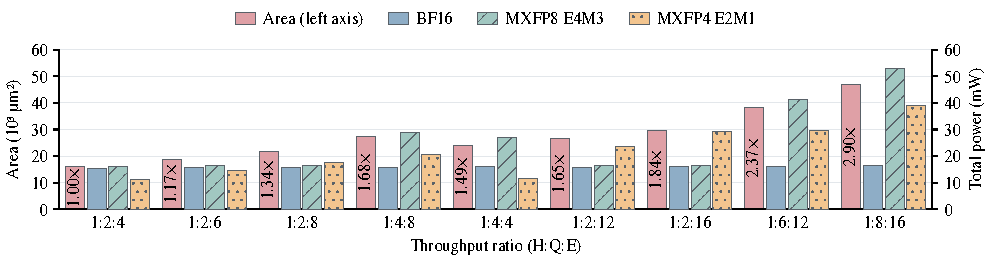
\includegraphics[width=\textwidth]{dp_ratio_area_power.pdf}
\caption{Synthesized area and total power of the nine throughput-ratio configurations. Area bars use the left axis, with labels indicating ratios relative to $1:2:4$; power bars for the three precision modes use the right axis (mW).}
\label{fig:ratio4_costs}
\end{figure*}
% END REVIEW PAIR: 04_evaluation.tex

% BEGIN REVIEW PAIR: 06_workload.tex
\section{Case study:Workload-Driven Throughput-Ratio Analysis}
\label{sec:workload}

The benefit of low-precision expansion depends on the trade-off among per-core throughput, deployment density, and workload precision composition. We compare $1:2:4$, $1:2:6$, $1:2:8$, and $1:4:8$ under a common area budget, identify their latency- and energy-optimal regions, and assess their applicability using compute-intensive DeepSeek prefill workloads.

\begin{figure}[!t]
\centering
\includegraphics[width=\columnwidth]{k4_n12_prefill_comparison.png}
\caption{Equal-area ratio selection for (a) compute latency with integer core deployment and (b) DP compute energy. Each region is labeled by its optimal H:Q:E ratio and geometric area fraction. The inset illustrates H/Q/E = 20\%/30\%/50\%. Trajectories are model-derived DeepSeek prefill workloads: dashed/solid lines use routed-expert W4A8/W4A4, with other computations unchanged. Arrows follow contexts of 1K, 4K, 16K, 64K, 256K, 512K, and 1M; filled markers denote 1M. NVFP4 energy uses the MXFP4 power proxy.}
\label{fig:k4_time_prefill}
\end{figure}

\subsection{Throughput Model Under an Equal-Area Constraint}
\label{sec:k4_area}

Each AI compute core contains an $m=n=16$ DP array. Using the compute-unit area breakdown reported by Luo et al.~\cite{luo2024hifloat8area} and the published core count~\cite{huawei950} as references, we set $\alpha=0.30$ and $N_0=36$ to construct an equivalent area budget, rather than reproduce an actual chip area.

For ratio $j$, let $a_j$ be the area of one DP and $A_{T,j}=256a_j$ the array area; subscript 0 denotes $1:2:4$. The baseline core area, fixed peripheral area, and total budget are
\begin{equation}
A_{C,0}=\frac{A_{T,0}}{\alpha},\quad
A_O=A_{C,0}-A_{T,0},\quad
A_{\mathrm{bud}}=N_0A_{C,0}.
\label{eq:k4_area_definition}
\end{equation}
Keeping peripheral area $A_O$ fixed per core, complete cores are deployed within $A_{\mathrm{bud}}=496.59$\,mm$^2$:
\begin{equation}
n_j=\left\lfloor\frac{A_{\mathrm{bud}}}{A_O+A_{T,j}}\right\rfloor.
\label{eq:core_area_budget}
\end{equation}
Let $d\in\{H,Q,E\}$ index precision, $m_{j,d}$ denote MACs per cycle per DP, and $p_{j,d}$ denote the full-throughput active power measured in Section V. Counting two FLOPs per MAC at clock frequency $f=1$\,GHz, the deployed peak throughput and DP active power are
\begin{equation}
C_{j,d}=2f\,256n_jm_{j,d},\qquad
P_{j,d}=256n_jp_{j,d}.
\label{eq:k4_capacity_power}
\end{equation}

The fixed area budget accommodates 36, 34, 32, and 29 cores for the four ratios, respectively (Table~\ref{tab:k4_absolute}). Low-precision expansion raises per-core throughput but reduces deployment density; its net benefit depends on whether low-precision acceleration offsets the loss of H throughput.

% Retained for the English manuscript chapters awaiting revision.
\begin{table}[!t]
\centering
\caption{Area-constrained N12 deployment. $A_C$: core area (mm$^2$); $C$: TFLOP/s; $P$: DP-only power (W).}
\label{tab:k4_absolute}
\begingroup\footnotesize\setlength{\tabcolsep}{3pt}
\input{tables/hardware_compact_table.tex}
\endgroup
\end{table}


\subsection{Optimal Regions for Mixed-Precision Workloads}
\label{sec:k4_simplex}

Let $F=\sum_d F_d$ be the total useful H/Q/E GEMM work, with $x_d=F_d/F$ and $\sum_d x_d=1$. Assuming precision phases execute sequentially and fully utilize all cores, compute latency and DP energy are
\begin{align}
T_j&=F\sum_d\frac{x_d}{C_{j,d}},&
C_{\mathrm{eff},j}&=\frac{F}{T_j},
\label{eq:k4_time}\\
\mathcal E_j&=\sum_d P_{j,d}\frac{Fx_d}{C_{j,d}}.
\label{eq:k4_energy}
\end{align}
We evaluate 5,151 compositions at one-percentage-point intervals over the H/Q/E triangle, minimizing $T_j$ and $\mathcal E_j$ separately. For fixed $F$, both are linear in $\boldsymbol x$, so equal-cost conditions between ratios define straight region boundaries (Fig.~\ref{fig:k4_time_prefill}). Labels report the geometric fraction of the triangle where each ratio is optimal, not hardware area or application probability. Following grid lines parallel to the opposite sides gives the H/Q/E FLOP shares of a point, which sum to $100\%$.

H-, E-, and Q-heavy regions favor $1:2:4$, $1:2:8$, and $1:4:8$, respectively. For H/E mixtures with little Q work, $1:2:6$ balances E acceleration against lost H throughput with a smaller area increment. Latency benefits depend on each phase's $F_d/C_{j,d}$, rather than an individual FLOP share. Energy per FLOP, $P_{j,d}/C_{j,d}=p_{j,d}/(2fm_{j,d})$, is independent of core count, so the latency- and energy-optimal regions differ.

\subsection{DeepSeek Precision Demand and Ratio Selection}
\label{sec:k4_prefill}

Using official configurations~\cite{deepseekv4,deepseekv4flashsource,deepseekv4prosource,deepseekv41source}, we count cold-prefill work for V4-Flash, V4-Pro, and V4.1-Flash at batch size 1 across seven contexts from 1K to 1M. GEMMs contribute $2MNK$ FLOPs; only active experts are counted, with sparse/compressed attention and V4.1 CED and index reuse included. BF16 attention and grouped output projections map to H; W4A8 expert computation and FP8 projections to Q; and MXFP4 indexer dot products to E. The NVFP4 W4A4 mapping moves only routed experts from FP8 to FP4. Each mapping contains 21 points and covers 97.11\%--99.37\% of GEMM work.

All W4A8 points favor $1:4:8$ for both latency and energy. With W4A4 experts, V4-Flash's energy optimum shifts to $1:2:8$ at 512K and its latency optimum at 1M; the other two models retain $1:4:8$ through 1M. At the V4-Flash 1M point, $1:2:8$ improves latency and estimated energy by 1.45\% and 2.03\%, respectively, relative to $1:4:8$, indicating limited gains near the boundary. Thus, $1:4:8$ is generally favored by the representative workloads evaluated here. If FP4 execution extends to attention and other operations as contexts grow longer, $1:2:8$ may become more attractive.
% END REVIEW PAIR: 06_workload.tex

% BEGIN REVIEW PAIR: 07_conclusion.tex
\section{Conclusion}
\label{sec:conclusion}

This paper proposes a microarchitecture for shared multi-precision dot-product operations, decoupling multi-precision coverage from capacity expansion for low-precision computations. The baseline architecture reuses multi-precision compute paths through unified decoding, segmented multiplication, hierarchical alignment, and fused output stages. Dedicated low-precision optimization units further prune unnecessary high-precision resources, achieving a 3× improvement in energy efficiency compared to the Ten-Four~\cite{rout2026tenfourv2} multi-precision design, while maintaining competitive area efficiency. The architecture supports internal reduction expansion along the $K$ dimension and independent output combination along the $N$ dimension. At equivalent peak performance, the evaluated $K$-expansion scheme offers a smaller area footprint and lower active power consumption for low-precision operations, while exhibiting a more moderate growth in bandwidth requirements under typical Weight-Stationary (WS) dataflow and matrix-size conditions.

Furthermore, under a fixed-area constraint, this work evaluates the impact of dot-product units within the context of AI chip systems and real-world computational workloads. By identifying the optimal operating regimes for four distinct configuration ratios—and analyzing the deployment of three DeepSeek mixed-precision models—we determine that a $1:4:8$ ratio is well-suited for W4A8 expert-based deployments, while certain W4A4 long-context configurations favor a $1:2:8$ ratio (with diminishing returns near the boundaries). Our findings suggest that configuration ratios should be determined based on the workload distribution across precisions and the time spent during the post-deployment compute-evaluation phase; specifically, low-precision acceleration can compensate for reduced deployment density, and energy consumption should be evaluated independently. Neither weight bit-width nor peak performance alone is sufficient to dictate the optimal ratio. By exploring various configuration ratios within the dot-product microarchitecture—analyzing both $K$-expansion and $N$-combination approaches—this paper provides a framework for selecting and designing compute-ratio architectures for future AI chips, based on latency and energy-efficiency analysis across real-world workloads and their evolving usage scenarios.
% END REVIEW PAIR: 07_conclusion.tex


\section*{Content Generated by AI}
OpenAI Codex assisted with EDA scripting, interpretation of source code and microarchitecture, experimental modeling, data analysis, plotting scripts, and manuscript organization, drafting, and translation. The authors are responsible for the adopted scripts, results, and all claims in this paper.

\clearpage
\setcounter{DACreferencepage}{\value{page}}
\ifnum\value{DACreferencepage}>7\relax
  \PackageWarningNoLine{DAC2027}{Main text exceeds six pages}%
\fi
\typeout{DAC2027: References start on page \thepage}
\bibliographystyle{IEEEtran}
\bibliography{references/references}
\end{document}
